% =====================================================================
%  Equivalence of the interband absorption integral with Rosei's EDJDOS
%  Side-by-side reconciliation for the gold X (and L) critical points.
%  Compile:  pdflatex (run twice for cross-references)  or  latexmk -pdf
% =====================================================================
\documentclass[11pt]{article}

% ---- Fonts & encoding ------------------------------------------------
\usepackage[T1]{fontenc}
\usepackage[utf8]{inputenc}
% amsmath/amssymb must precede newtxmath to avoid the \Bbbk redefinition clash
\usepackage{amsmath,amssymb,mathtools,bm}
\usepackage{newtxtext,newtxmath}
\usepackage[scaled=0.92]{helvet}
\usepackage{microtype}

% ---- Page geometry ---------------------------------------------------
\usepackage[margin=2.3cm,top=2.2cm]{geometry}
\setlength{\parskip}{0.45em}
\setlength{\parindent}{0pt}

% ---- Colour, tables, boxes ------------------------------------------
\usepackage[table,dvipsnames]{xcolor}
\definecolor{workcol}{HTML}{1F4E79}   % deep blue  -- this work
\definecolor{roseicol}{HTML}{8C3B2E}  % brick red  -- Rosei (1975)
\definecolor{worklite}{HTML}{EAF1F8}
\definecolor{roseilite}{HTML}{F7ECEA}
\definecolor{steplite}{HTML}{E9EDF2}
\definecolor{keylite}{HTML}{FBF6E9}
\definecolor{keyrule}{HTML}{B8860B}
\definecolor{warncol}{HTML}{7A1F1F}

\usepackage{colortbl}
\usepackage{booktabs}
\usepackage{array}
\usepackage{tabularx}
\usepackage{longtable}
\newcolumntype{Y}{>{\centering\arraybackslash}X}
\newcolumntype{Z}{>{\centering\arraybackslash}p{0.452\textwidth}}

\usepackage[most]{tcolorbox}
\tcbuselibrary{skins,breakable,raster}

\usepackage{enumitem}
\setlist{nosep,leftmargin=1.4em}
\usepackage{caption}
\captionsetup{font=small,labelfont={bf,sf,color=workcol}}

\usepackage{tikz}
\usetikzlibrary{calc}

% ---- Section styling -------------------------------------------------
\usepackage{titlesec}
\titleformat{\section}{\normalfont\large\bfseries\sffamily\color{workcol}}
  {\thesection}{0.7em}{}
\titleformat{\subsection}{\normalfont\normalsize\bfseries\sffamily\color{workcol!82!black}}
  {\thesubsection}{0.6em}{}
\titlespacing*{\section}{0pt}{1.4em}{0.5em}

% ---- Hyperlinks ------------------------------------------------------
\usepackage[colorlinks=true,linkcolor=workcol,citecolor=workcol,urlcolor=workcol]{hyperref}
\usepackage{cleveref}

% ---- Macros ----------------------------------------------------------
\newcommand{\kperp}{k_{\perp}}
\newcommand{\kpar}{k_{\parallel}}
\newcommand{\hw}{\hbar\omega}
\newcommand{\EgX}{\mathcal{E}_{g}^{X}}
\newcommand{\EgL}{\mathcal{E}_{g}^{L}}
\newcommand{\Dc}{\mathcal{D}}
\newcommand{\Flu}{\mathcal{F}_{l\to u}}
\newcommand{\Jc}{\mathcal{J}}
\newcommand{\Dlu}{D_{l\to u}}
\newcommand{\Ic}{\mathcal{I}_{l\to u}}
\newcommand{\Ab}{\bar{A}}
\newcommand{\Bb}{\bar{B}}
\newcommand{\wXsix}{\hbar\omega_{X_6^-}}
\newcommand{\wXseven}{\hbar\omega_{X_7^+}}
% Rosei equation reference, coloured for instant recognition
\newcommand{\Rq}[1]{\textcolor{roseicol}{\textnormal{(#1)}}}
\newcommand{\This}{\textcolor{workcol}{\textsf{This work}}}
\newcommand{\GRW}{\textcolor{roseicol}{\textsf{GRW\,1975}}}

% ---- tcolorbox styles ------------------------------------------------
\newtcolorbox{keybox}[1][Result]{
  enhanced, breakable, colback=keylite, colframe=keyrule,
  boxrule=0.9pt, arc=2pt, left=8pt,right=8pt,top=6pt,bottom=6pt,
  fonttitle=\bfseries\sffamily, coltitle=warncol,
  attach boxed title to top left={xshift=8pt,yshift=-3mm},
  boxed title style={colback=keylite,colframe=keyrule,boxrule=0.6pt,arc=1pt},
  title={#1}}

\newtcolorbox{workpanel}{
  enhanced, colback=worklite, colframe=workcol, boxrule=0.8pt, arc=2pt,
  left=7pt,right=7pt,top=12pt,bottom=6pt,
  overlay={\node[anchor=north west,font=\bfseries\sffamily\small,
     text=white,fill=workcol,inner sep=2.5pt,rounded corners=1pt]
     at ([xshift=6pt,yshift=2pt]frame.north west) {This work};}}

\newtcolorbox{roseipanel}{
  enhanced, colback=roseilite, colframe=roseicol, boxrule=0.8pt, arc=2pt,
  left=7pt,right=7pt,top=12pt,bottom=6pt,
  overlay={\node[anchor=north west,font=\bfseries\sffamily\small,
     text=white,fill=roseicol,inner sep=2.5pt,rounded corners=1pt]
     at ([xshift=6pt,yshift=2pt]frame.north west) {Guerrisi--Rosei--Winsemius 1975};}}

% =====================================================================
\begin{document}

% ---- Title block -----------------------------------------------------
\begin{center}
  {\sffamily\bfseries\LARGE\color{workcol}
   Equivalence of the Interband Absorption Integral\\[2pt]
   with Rosei's Energy-Distributed Joint Density of States}\\[8pt]
  {\large A step-by-step reconciliation at the gold $X$ and $L$ critical points}\\[10pt]
  {\normalsize Ben Shpigel \quad\textbullet\quad Ben-Gurion University of the Negev}\\[2pt]
  {\small\itshape \today}
\end{center}

\begin{tcolorbox}[colback=gray!6,colframe=gray!55,boxrule=0.6pt,arc=2pt,
  left=10pt,right=10pt,top=7pt,bottom=7pt]
\small
\textbf{Abstract.} We carry the interband contribution to $\varepsilon_2(\hw,T)$ of gold from
Fermi's golden rule down to a one-dimensional energy integral, retaining every
$\hbar^2/2m$ factor and the full non-equilibrium occupation
$f(E_l)\,[1-f(E_u)]$. We then place this reduction \emph{line by line} beside the
energy-distributed joint-density-of-states (EDJDOS) expression of Guerrisi, Rosei \&
Winsemius, \textit{Phys.\ Rev.\ B} \textbf{12}, 557 (1975) [Eqs.~\Rq{1}--\Rq{9}].
The two integrands are shown to be the \emph{same function of} $(E,\omega)$: they share
the identical shape-carrying factor $\kpar^{-1}(E,\omega)$ and the identical integration
limits, and differ only by (i) a multiplicative constant $16\pi^3\Flu/\hbar^2$ that is
independent of $E$ and $\omega$ and is absorbed into the overall fitted scale, and (ii)
the valence-band-full approximation $f(E_l)\!\to\!1$, under which our statistical factor
collapses to Rosei's $[1-f(E)]$. Finally we examine two of Rosei's printed display
equations, \Rq{6} and \Rq{8}, and show on dimensional, geometric, and internal-consistency
grounds that the corrected upper integration limit must carry \emph{perpendicular}, not
parallel, effective masses.
\end{tcolorbox}

% =====================================================================
\section{Setup, notation, and the claim}
\label{sec:setup}

Both treatments describe the same physical process: a vertical (direct, $\mathbf
k_u=\mathbf k_l\equiv\mathbf k$) transition from the filled $d$-derived band $l$ to the
$sp$ band $u$ near the $X$ point of gold, under rotational symmetry about the $\Gamma X$
axis. Rosei's quadratic dispersions, measured from the Fermi level, are his Eqs.~\Rq{1}
and~\Rq{2}:
%
\begin{align}
E \;=\; \hbar\omega_u
   &= \wXsix + \frac{\hbar^2\kperp^2}{2m_{u\perp}} - \frac{\hbar^2\kpar^2}{2m_{u\|}},
   &&\text{\Rq{1}\quad(saddle: $+\kperp^2$, $-\kpar^2$)}\label{eq:Eu}\\[2pt]
E-\hw \;=\; \hbar\omega_l
   &= -\wXseven - \frac{\hbar^2\kperp^2}{2m_{l\perp}} - \frac{\hbar^2\kpar^2}{2m_{l\|}},
   &&\text{\Rq{2}\quad(maximum: $-\kperp^2$, $-\kpar^2$)}\label{eq:El}
\end{align}
%
Throughout we use the compact curvature coefficients
%
\begin{equation}
A_i=\frac{\hbar^2}{2m_{i\perp}},\qquad
B_i=\frac{\hbar^2}{2m_{i\|}},\qquad i=l,u,
\label{eq:AB}
\end{equation}
%
so that the interband (transition) energy and the vertical gap are
%
\begin{equation}
\Omega_{lu}(\mathbf k)\equiv\hbar\omega_u-\hbar\omega_l
=\EgX+\Ab\,\kperp^2+\Bb\,\kpar^2,
\qquad
\Ab=A_u+A_l,\quad \Bb=B_l-B_u,\quad \EgX=\wXsix+\wXseven .
\label{eq:Omega}
\end{equation}
%
The minus sign on $\kpar^2$ in \eqref{eq:Eu} makes $u$ a saddle, so $\Omega_{lu}$ is a
saddle in $\mathbf k$ and the constant-energy-difference surface (CEDS)
$\Omega_{lu}=\hw$ is an \emph{open} hyperboloid; this is the origin of the sub-gap tail
treated in \cref{sec:limits}. The companion $L$ point differs only in the sign of the
upper-band $\kpar^2$ curvature and is collected in \cref{sec:limits}.

\paragraph{The two integrands to be reconciled.} The object of this note is to prove the
identity boxed below.
%
\begin{keybox}[Claim]
The absorption integrand obtained here by an explicit change of variables,
\[
\varepsilon''(\omega)\ \propto\ \int f(E-\hw)\,[1-f(E)]\,\Jc(E)\,dE,
\qquad
\Jc(E)=\left.\frac{2\pi\kperp}{|\det J|}\right|_{\Delta=\hw},
\]
and Rosei's EDJDOS integrand [Eqs.~\Rq{4}, \Rq{7}],
\[
\varepsilon_2^{\text{Rosei}}(\omega)\ \propto\ \int [1-f(E)]\,\Dlu(E,\hw)\,dE,
\qquad
\Dlu(E,\hw)=\bigl(8\pi^2\hbar^2\bigr)^{-1}\Flu\,\kpar^{-1},
\]
describe the \emph{same} spectral function. Explicitly,
\[
\boxed{\ \Jc(E)=\underbrace{\frac{16\pi^{3}\Flu}{\hbar^{2}}}_{\text{const.\ in }E,\,\omega}\,\Dlu(E,\hw)\ }
\qquad\text{and}\qquad
f(E_l)\,[1-f(E_u)]\ \xrightarrow{\,f(E_l)\to1\,}\ [1-f(E)].
\]
\end{keybox}

% =====================================================================
\section{The two reductions, line by line}
\label{sec:ledger}

We first display the logical skeletons in parallel, then carry out the one nontrivial
common step --- the Jacobian --- in \cref{sec:jacobian}.

{\renewcommand{\arraystretch}{1.42}
\setlength{\tabcolsep}{6pt}
\setlength{\LTpre}{6pt}\setlength{\LTpost}{4pt}
\arrayrulecolor{gray!55}
\begin{longtable}{@{}ZZ@{}}
\rowcolor{steplite}\multicolumn{2}{@{}>{\columncolor{steplite}}c@{}}{%
  \footnotesize\sffamily\bfseries STEP 0 \;\textbullet\; Starting point}\\*
\cellcolor{worklite}$\displaystyle \varepsilon''\propto\!\iiint\! f(E_l)[1-f(E_u)]\delta(\Omega_{lu}\!-\!\hw)d^3k$ &
\cellcolor{roseilite}$\displaystyle \varepsilon_2=\frac{8\pi^2e^2\hbar^4}{3m^2(\hw)^2}\!\sum_{P}|P_P|^2 g_P$ \;\Rq{9}\\*
\cellcolor{worklite}\footnotesize golden rule, explicit occupation &
\cellcolor{roseilite}\footnotesize $g_P=N_P\,\Ic$, with $\Ic$ from \Rq{7}\\

\rowcolor{steplite}\multicolumn{2}{@{}>{\columncolor{steplite}}c@{}}{%
  \footnotesize\sffamily\bfseries STEP 1 \;\textbullet\; Exploit cylindrical symmetry}\\*
\cellcolor{worklite}$\displaystyle d^3k\to 2\pi\kperp\,d\kperp\,d\kpar$ &
\cellcolor{roseilite}$\displaystyle d^3k\to 2\pi\kperp\,d\kperp\,d\kpar$\\*
\cellcolor{worklite}\footnotesize same measure &
\cellcolor{roseilite}\footnotesize same measure (Ref.~10 procedure)\\

\rowcolor{steplite}\multicolumn{2}{@{}>{\columncolor{steplite}}c@{}}{%
  \footnotesize\sffamily\bfseries STEP 2 \;\textbullet\; Change variables $(\kperp,\kpar)\to(E,\,\cdot)$}\\*
\cellcolor{worklite}$\displaystyle E\equiv E_u,\quad \Delta\equiv E_u-E_l$ &
\cellcolor{roseilite}$\displaystyle E\equiv E_u,\quad \Omega\equiv E_u-E_l$\\*
\cellcolor{worklite}\footnotesize $\Delta=\EgX+\Ab\kperp^2+\Bb\kpar^2$ &
\cellcolor{roseilite}\footnotesize identical map; $\Omega_{lu}=0$ is \Rq{3}\\

\rowcolor{steplite}\multicolumn{2}{@{}>{\columncolor{steplite}}c@{}}{%
  \footnotesize\sffamily\bfseries STEP 3 \;\textbullet\; Jacobian of the map (see \S\ref{sec:jacobian})}\\*
\cellcolor{worklite}$\displaystyle |\det J|=4\kperp\kpar\,\Dc$ &
\cellcolor{roseilite}$\displaystyle \Dc=\Bigl(\tfrac{\hbar^2}{2}\Bigr)^{2}\Flu^{-2}$\\*
\cellcolor{worklite}\footnotesize $\Dc=A_uB_l+A_lB_u$ (mass constant) &
\cellcolor{roseilite}\footnotesize folded into $\Flu$, Eq.~\Rq{5}\\

\rowcolor{steplite}\multicolumn{2}{@{}>{\columncolor{steplite}}c@{}}{%
  \footnotesize\sffamily\bfseries STEP 4 \;\textbullet\; Collapse the energy-conserving $\delta$}\\*
\cellcolor{worklite}$\displaystyle \Jc(E)=\frac{2\pi\kperp}{4\kperp\kpar\Dc}=\frac{2\pi\Flu^{2}}{\hbar^{4}\,\kpar}$ &
\cellcolor{roseilite}$\displaystyle \Dlu=\frac{\Flu}{8\pi^{2}\hbar^{2}\,\kpar}$ \;\Rq{4}\\*
\cellcolor{worklite}\footnotesize shape carried entirely by $\kpar^{-1}(E,\omega)$ &
\cellcolor{roseilite}\footnotesize shape carried entirely by $\kpar^{-1}(E,\omega)$\\

\rowcolor{steplite}\multicolumn{2}{@{}>{\columncolor{steplite}}c@{}}{%
  \footnotesize\sffamily\bfseries STEP 5 \;\textbullet\; Statistical weight}\\*
\cellcolor{worklite}$\displaystyle f(E-\hw)\,[1-f(E)]$ &
\cellcolor{roseilite}$\displaystyle [1-f(E)]$ \;(\Rq{7})\\*
\cellcolor{worklite}\footnotesize general / non-equilibrium-ready &
\cellcolor{roseilite}\footnotesize $f(E_l)\to1$ limit (filled $d$ band)\\
\bottomrule
\end{longtable}}

Reading down the two columns, every line is either identical or differs by a constant
prefactor. Only Steps~3--5 require argument; we supply each in turn.

% =====================================================================
\section{Step 3 --- the Jacobian is the band-curvature determinant}
\label{sec:jacobian}

With $E=E_u$ from \eqref{eq:Eu} and $\Delta=\Omega_{lu}$ from \eqref{eq:Omega}, the
Jacobian matrix of $(E,\Delta)$ with respect to $(\kperp,\kpar)$ is
%
\begin{equation}
J=\begin{pmatrix}
\partial_{\kperp}E & \partial_{\kpar}E\\[3pt]
\partial_{\kperp}\Delta & \partial_{\kpar}\Delta
\end{pmatrix}
=\begin{pmatrix}
2A_u\kperp & -2B_u\kpar\\[3pt]
2\Ab\,\kperp & 2\Bb\,\kpar
\end{pmatrix},
\end{equation}
%
whose determinant factors the momenta out cleanly:
%
\begin{equation}
\det J = 4\kperp\kpar\bigl(A_u\Bb+B_u\Ab\bigr)
       = 4\kperp\kpar\bigl[A_u(B_l-B_u)+B_u(A_u+A_l)\bigr]
       = 4\kperp\kpar\,(A_uB_l+A_lB_u).
\end{equation}
%
Hence
%
\begin{equation}
|\det J| = 4\,\kperp\kpar\,\Dc,
\qquad
\boxed{\ \Dc\equiv A_uB_l+A_lB_u\ }
\label{eq:Ddef}
\end{equation}
%
is a pure effective-mass constant --- no $E$, $\omega$, or $k$ dependence. The factor of
$\kperp$ in the numerator measure $2\pi\kperp$ cancels the $\kperp$ in $|\det J|$, leaving
the entire spectral shape in the single surviving factor $\kpar^{-1}$. Expanding
\eqref{eq:Ddef} with \eqref{eq:AB},
%
\begin{equation}
\Dc=\Bigl(\tfrac{\hbar^2}{2}\Bigr)^{2}
\!\left(\frac{1}{m_{u\perp}m_{l\|}}+\frac{1}{m_{l\perp}m_{u\|}}\right)
=\Bigl(\tfrac{\hbar^2}{2}\Bigr)^{2}
\frac{m_{l\perp}m_{u\|}+m_{l\|}m_{u\perp}}{m_{l\perp}m_{l\|}m_{u\perp}m_{u\|}} .
\label{eq:Dexpand}
\end{equation}
%
Comparing the mass ratio in \eqref{eq:Dexpand} with Rosei's definition of $\Flu$
[Eq.~\Rq{5}],
%
\begin{equation}
\Flu=\left(\frac{m_{l\perp}m_{u\|}+m_{l\|}m_{u\perp}}{m_{l\perp}m_{l\|}m_{u\perp}m_{u\|}}\right)^{-1/2}
\quad\Longrightarrow\quad
\boxed{\ \Dc=\Bigl(\tfrac{\hbar^2}{2}\Bigr)^{2}\Flu^{-2}\ }.
\label{eq:bridge}
\end{equation}
%
\Cref{eq:bridge} is the bridge between the two notations: the determinant that my
change of variables produces is precisely the inverse square of the constant Rosei
defines. The two derivations have met.

% =====================================================================
\section{Step 4 --- the kernels coincide up to a constant}
\label{sec:kernel}

Insert \eqref{eq:bridge} into the kernel of Step~4. From $|\det J|=4\kperp\kpar\Dc$ and
$\Dc=(\hbar^2/2)^2\Flu^{-2}$,
%
\begin{equation}
\Jc(E)=\frac{2\pi\kperp}{4\kperp\kpar\,\Dc}
=\frac{\pi}{2\kpar}\,\Dc^{-1}
=\frac{\pi}{2\kpar}\Bigl(\tfrac{\hbar^2}{2}\Bigr)^{-2}\Flu^{2}
=\frac{2\pi\,\Flu^{2}}{\hbar^{4}\,\kpar}.
\label{eq:Jfinal}
\end{equation}
%
Dividing by Rosei's $\Dlu=\Flu\,(8\pi^2\hbar^2\kpar)^{-1}$ [Eq.~\Rq{4}], the
$\kpar^{-1}$ cancels exactly and the ratio is constant:
%
\begin{equation}
\frac{\Jc(E)}{\Dlu(E,\hw)}
=\frac{2\pi\Flu^{2}/(\hbar^{4}\kpar)}{\Flu/(8\pi^{2}\hbar^{2}\kpar)}
=2\pi\Flu^{2}\cdot\frac{8\pi^{2}\hbar^{2}}{\hbar^{4}\Flu}
=\frac{16\pi^{3}\Flu}{\hbar^{2}} .
\label{eq:ratio}
\end{equation}
%
\begin{keybox}[Identity of the kernels]
\[
\Jc(E)=\frac{16\pi^{3}\Flu}{\hbar^{2}}\;\Dlu(E,\hw),
\qquad\text{with}\qquad
\frac{16\pi^{3}\Flu}{\hbar^{2}}\ \text{independent of }E\text{ and }\omega .
\]
The only carrier of spectral shape, $\kpar^{-1}(E,\omega)$, is \emph{identical} in both;
the integrands differ by a global multiplicative constant and nothing else.
\end{keybox}

\subsection{Why the constant is not a discrepancy but a units bridge}

The prefactor $16\pi^3\Flu/\hbar^2$ is exactly what reconciles the apparent
``missing factor'' between the bare EDJDOS and Rosei's $\Dlu$. Since
$\Flu^{-2}$ has dimensions $(\text{mass})^{-2}$, $\Flu$ carries one power of mass, and
%
\begin{equation}
\left[\frac{\Flu}{\hbar^{2}}\right]
=\frac{\text{kg}}{(\text{J\,s})^{2}}=\frac{1}{\text{J}\,\text{m}^{2}}
=\left[\frac{2m}{\hbar^{2}}\right].
\label{eq:units}
\end{equation}
%
This is precisely the $\text{J}^{-1}\text{m}^{-2}$ by which Rosei's $\Dlu$ differs from a
fully normalized energy-distributed JDOS (dimensions
$[\text{vol}]^{-1}[\text{energy}]^{-2}=\text{m}^{-3}\text{J}^{-2}$). In words:
%
\begin{itemize}
\item Our $\Jc\propto\Flu^{2}/\kpar$ carries the dimensionally complete coefficient
      because every $\hbar^2/2m$ was retained explicitly through the Jacobian
      \eqref{eq:Ddef}.
\item Rosei pushed \emph{one} power of $2m/\hbar^2$ into his definition of $\Flu$ (leaving
      $\Flu^{1}$ in Eq.~\Rq{4}) and the rest into the overall normalization in front of
      $\varepsilon_2$ in Eq.~\Rq{9}. His $\Dlu$ is therefore a \emph{rescaled} EDJDOS,
      not the bare one.
\end{itemize}
%
Because $16\pi^3\Flu/\hbar^2$ is constant across the band, it is absorbed without trace
into the single overall amplitude of $\varepsilon_2$ --- the strengths $S_X,S_L$ of
Rosei's Eq.~\Rq{10} (the \texttt{Scale} parameter of the fit). \textbf{No spectral
information is created, lost, or shifted.}

% =====================================================================
\section{Step 5 --- the statistical factors agree}
\label{sec:occupation}

The full microscopic weight of a vertical transition is the product
``initial filled $\times$ final empty,''
%
\begin{equation}
f(E_l)\,[1-f(E_u)]=f(E-\hw)\,[1-f(E)],
\end{equation}
%
where the second equality uses $E_l=E-\hw$ from the change of variables. For ordinary
absorption the initial state $l$ is the $d$-derived band lying well below the Fermi
level: at the energies that contribute, $E_l\simeq-\wXseven\ll E_F$, so
%
\begin{equation}
f(E-\hw)=f(E_l)\xrightarrow{\,E_l\ll E_F\,}1 .
\end{equation}
%
Rosei's integrand $[1-f(E)]$ is thus the $f(E_l)\to1$ limit of ours; the bracket
``gives the probability that a state with energy $E$ in the upper band is empty,'' in his
words following Eq.~\Rq{7}. Retaining $f(E-\hw)$ explicitly --- as we do --- is the more
general form, and is mandatory once the bands are driven out of equilibrium (elevated
electronic temperature, pulsed excitation, or emission), where the initial-state
occupation is no longer unity. At equilibrium absorption the two coincide identically.

% =====================================================================
\section{Integration limits, line shape, and the $L$ partner}
\label{sec:limits}

The remaining content of Eqs.~\Rq{6}--\Rq{8} is the domain of $E$ and the
$E$-dependence of $\kpar$. Solving \eqref{eq:Eu} together with $\Omega_{lu}=\hw$ for the
in-plane momentum (eliminate $\kperp^2$) gives the dimensionally clean
%
\begin{equation}
\boxed{\ \kpar^{2}=\frac{1}{\Dc}\Bigl[A_u\,(\hw-\EgX)-\Ab\,(E-\wXsix)\Bigr]\ }
\tag{6$'$}
\label{eq:6prime}
\end{equation}
%
the corrected form of Rosei's Eq.~\Rq{6} (see \cref{sec:printed}). Equation
\eqref{eq:6prime} shows $\Dlu\propto\kpar^{-1}\propto(E_{\max}-E)^{-1/2}$: an integrable
inverse-square-root edge in $E$ at the $\kpar=0$ end. The positivity $\kpar^2\ge0$ fixes
the upper limit at $\kpar=0$,
%
\begin{equation}
E_{\max}=\wXsix+\frac{A_u}{\Ab}\,(\hw-\EgX)
       =\wXsix+\frac{m_{l\perp}}{m_{l\perp}+m_{u\perp}}\,(\hw-\EgX),
\label{eq:Emax}
\end{equation}
%
the corrected form of Rosei's Eq.~\Rq{8}. Because the saddle CEDS is \emph{open}, the
companion condition $\kperp^2\ge0$ does not bound $E$ from below; following Rosei the
lower limit is the thermal floor $E_{\min}=-20\,k_BT$, below which $[1-f(E,T)]$ kills the
integrand. The wide, thermally limited lower range makes the $X$ EDJDOS look steplike in
$E$, and the absorption rises smoothly through $\EgX=1.94$~eV with a near-exponential
sub-gap tail --- the defining $X$ signature.

\subsection{The $L$ point: the same machinery, one sign flipped}

At $L$ the upper band is an ellipsoid ($+\kpar^2$ curvature), so $\Bb_L=B_u+B_l$ and the
curvature determinant takes the \emph{difference} form
$\Dc_L=A_uB_l-A_lB_u$. Every step of \cref{sec:jacobian,sec:kernel} goes through verbatim
with $\Dc\to\Dc_L$. Now \emph{both} positivity conditions bound $E$, so the closed
ellipsoid yields a finite window
%
\begin{equation}
E_{\min}^{L}=\hbar\omega_{L_6^-}+\frac{B_u}{\Bb_L}(\hw-\EgL)
\ \le\ E\ \le\
E_{\max}^{L}=\hbar\omega_{L_6^-}+\frac{A_u}{\Ab_L}(\hw-\EgL),
\end{equation}
%
of width $\propto(\hw-\EgL)$. With $[1-f]\approx$ const across the narrow near-onset
window, $\Ic^{L}\propto\int_{E_{\min}^L}^{E_{\max}^L}(E_{\max}^L-E)^{-1/2}dE
=2\sqrt{E_{\max}^L-E_{\min}^L}\propto\sqrt{\hw-\EgL}$ --- the textbook $M_0$ inverse-square-root
edge $\varepsilon_2\propto\sqrt{\hw-\EgL}$, a sharp onset at $\EgL=2.45$~eV with no
sub-gap tail.

\begin{figure}[h]
\centering
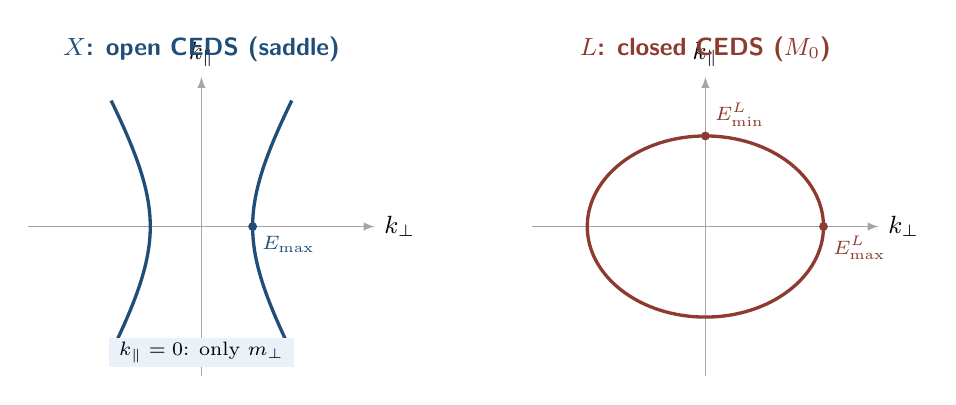
\begin{tikzpicture}[scale=1.0,>=latex]
  % ---------- X panel : open hyperbola (saddle) -------------------
  \begin{scope}[shift={(0,0)}]
    \draw[->,gray!70] (-2.2,0)--(2.2,0) node[right,black]{\small $\kperp$};
    \draw[->,gray!70] (0,-1.9)--(0,1.9) node[above,black]{\small $\kpar$};
    % hyperbola  kperp = a sqrt(1 + kpar^2/c^2)  (two branches)
    \draw[workcol,very thick,domain=-1.6:1.6,samples=60,smooth]
        plot ({0.65*sqrt(1+(\x*\x)/(1.1*1.1))},\x);
    \draw[workcol,very thick,domain=-1.6:1.6,samples=60,smooth]
        plot ({-0.65*sqrt(1+(\x*\x)/(1.1*1.1))},\x);
    \fill[workcol] (0.65,0) circle (1.6pt);
    \node[workcol,below right,font=\scriptsize] at (0.65,0) {$E_{\max}$};
    \node[font=\scriptsize,fill=worklite,inner sep=1.5pt] at (0,-1.6)
        {\;$\kpar=0$: only $m_\perp$\;};
    \node[workcol,font=\bfseries\sffamily\small] at (0,2.25)
        {$X$: open CEDS (saddle)};
  \end{scope}
  % ---------- L panel : closed ellipse (M0) -----------------------
  \begin{scope}[shift={(6.4,0)}]
    \draw[->,gray!70] (-2.2,0)--(2.2,0) node[right,black]{\small $\kperp$};
    \draw[->,gray!70] (0,-1.9)--(0,1.9) node[above,black]{\small $\kpar$};
    \draw[roseicol,very thick] (0,0) ellipse (1.5 and 1.15);
    \fill[roseicol] (1.5,0) circle (1.6pt);
    \fill[roseicol] (0,1.15) circle (1.6pt);
    \node[roseicol,below right,font=\scriptsize] at (1.5,0) {$E_{\max}^{L}$};
    \node[roseicol,above right,font=\scriptsize] at (0,1.15) {$E_{\min}^{L}$};
    \node[roseicol,font=\bfseries\sffamily\small] at (0,2.25)
        {$L$: closed CEDS ($M_0$)};
  \end{scope}
\end{tikzpicture}
\caption{Constant-energy-difference surfaces $\Omega_{lu}=\hw$ in the $(\kperp,\kpar)$
plane. The upper integration limit $E_{\max}$ sits at $\kpar=0$ on the $\kperp$ axis,
where the parallel curvatures $B_u,B_l$ have dropped out of both constraints --- hence
$E_{\max}$ depends only on the \emph{perpendicular} masses (\cref{sec:printed}). At $X$
the surface is an open hyperbola (sub-gap tail); at $L$ it is a closed ellipse (sharp
$M_0$ onset).}
\label{fig:ceds}
\end{figure}

\begin{center}\small
\renewcommand{\arraystretch}{1.25}
\begin{tabular}{@{}l c c@{}}
\toprule
 & \textbf{\textcolor{workcol}{$X$ (saddle, $M_1$)}} & \textbf{\textcolor{roseicol}{$L$ (ellipsoid, $M_0$)}}\\
\midrule
upper-band $\kpar^2$ sign      & $-B_u$ (saddle)        & $+B_u$ (ellipsoid)\\
CEDS topology                  & open hyperboloid       & closed ellipsoid\\
curvature determinant          & $\Dc_X=A_uB_l+A_lB_u$  & $\Dc_L=A_uB_l-A_lB_u$\\
$E$ range                      & $[-20k_BT,\ E_{\max}]$  & $[E_{\min}^L,\ E_{\max}^L]$ finite\\
edge in $E$                    & steplike (box)         & inverse-$\sqrt{\ }$\\
edge in $\hbar\omega$          & smooth, sub-gap tail   & sharp $\sqrt{\hw-\EgL}$\\
onset                          & $1.94$~eV              & $2.45$~eV\\
\bottomrule
\end{tabular}
\end{center}

% =====================================================================
\section{Two printed equations of Rosei, examined}
\label{sec:printed}

Asserting that a seminal paper contains a slip demands proof, not assertion. We examine
Eqs.~\Rq{6} and \Rq{8} as printed and show, on three independent grounds, what the
corrected forms must be. We are careful to separate a \emph{shorthand} (constants
reshuffled, harmless) from a \emph{transcription error} (wrong masses, consequential).

\subsection{Eq.~\Rq{6}: a dimensional shorthand, correct masses}

As printed, Rosei's Eq.~\Rq{6} reads
%
\begin{equation}
\kpar=\left(\hw-\wXseven+\frac{\hbar^2}{2m_{l\perp}}\bigl(\wXsix-E\bigr)
            -\frac{\hbar^2}{2m_{u\perp}}E\right)^{1/2}.
\tag{6, as printed}
\end{equation}
%
Read literally in SI, the bracket adds an energy ($\hw-\wXseven$) to terms of the form
$\tfrac{\hbar^2}{2m}\times\text{energy}$, which carry dimensions
$(\text{J}\,\text{m}^2)\times\text{J}=\text{J}^2\text{m}^2$; the sum cannot equal
$\kpar^2\sim\text{m}^{-2}$. For the bracket to have dimension $\text{m}^{-2}$ the mass
coefficients must read $2m/\hbar^2$, not $\hbar^2/2m$, and an overall $\Dc^{-1}$ must
multiply the bracket. The dimensionally consistent statement is exactly
\eqref{eq:6prime}. \emph{Crucially, the masses in Eq.~\Rq{6} are the perpendicular ones,}
$m_{l\perp}$ and $m_{u\perp}$ --- which is correct, since by \eqref{eq:6prime}
$\kpar^2$ depends only on $A_u,A_l$. We therefore read Eq.~\Rq{6} as Rosei's own
shorthand, in which the $2m/\hbar^2$ constants and the determinant are folded away into
$\Flu$ and the overall scale (consistent with the momenta being quoted ``in units of
$\pi/4a$'' in his Fig.~3). The spectral content --- $\kpar$ linear-in-$E$, producing the
$(E_{\max}-E)^{-1/2}$ edge --- is unchanged.

\subsection{Eq.~\Rq{8}: parallel masses where perpendicular masses are required}

As printed, Rosei's upper limit is his Eq.~\Rq{8},
%
\begin{equation}
E_{\max}=\wXsix+\bigl(\wXseven+\wXsix-\hw\bigr)\,
         \frac{m_{u\|}}{m_{l\|}-m_{u\|}}
       =\wXsix-(\hw-\EgX)\,\frac{m_{u\|}}{m_{l\|}-m_{u\|}},
\tag{8, as printed}
\end{equation}
%
which carries the \emph{parallel} masses $m_{u\|},m_{l\|}$. This cannot be correct, for
three independent reasons.

\begin{enumerate}[label=\textbf{(\roman*)}]
\item \textbf{Internal inconsistency with Eq.~\Rq{6}.}
The upper limit is, by definition, the $\kpar=0$ root of the very relation in
Eq.~\Rq{6}. But Eq.~\Rq{6} contains \emph{only} the perpendicular masses
$m_{l\perp},m_{u\perp}$. A root of an equation in $\{m_{l\perp},m_{u\perp}\}$ cannot
introduce $\{m_{u\|},m_{l\|}\}$. Equations \Rq{6} and \Rq{8} of the same paper are thus
mutually inconsistent as printed; one of them has the wrong subscripts, and by (ii) it is
\Rq{8}.

\item \textbf{Geometric necessity.}
Set $\kpar=0$ directly in the two defining surfaces \eqref{eq:Eu} and
$\Omega_{lu}=\hw$:
\[
E_{\max}=\wXsix+A_u\kperp^2,\qquad
\hw=\EgX+\Ab\,\kperp^2\ \Rightarrow\ \kperp^2=\frac{\hw-\EgX}{\Ab}.
\]
Neither equation contains $B_u$ or $B_l$ once $\kpar=0$: the parallel curvatures have
literally dropped out. Therefore (cf.\ \cref{fig:ceds})
\[
E_{\max}=\wXsix+\frac{A_u}{\Ab}(\hw-\EgX)
        =\wXsix+\frac{m_{l\perp}}{m_{l\perp}+m_{u\perp}}(\hw-\EgX),
\]
a function of the \emph{perpendicular} masses alone. The appearance of $m_{u\|},m_{l\|}$
in Eq.~\Rq{8} is structurally impossible for a $\kpar=0$ edge.

\item \textbf{The printed coefficient is out of physical range.}
The exact slope is the manifest fraction
\[
\frac{A_u}{\Ab}=\frac{A_u}{A_u+A_l}\in(0,1)\qquad(\text{since }0<A_u<\Ab),
\]
numerically $\dfrac{m_{l\perp}}{m_{l\perp}+m_{u\perp}}=\dfrac{0.19}{0.19+0.31}=0.38$ with
Rosei's $X$ masses. The printed coefficient instead evaluates to
\[
\frac{m_{u\|}}{m_{l\|}-m_{u\|}}=\frac{0.40}{0.15-0.40}=-1.6,
\]
\emph{negative and of magnitude exceeding unity}: it arises from the near-cancellation
$m_{l\|}-m_{u\|}$ in the denominator and cannot represent a positive edge fraction in
$(0,1)$. A slope of $-1.6$ would place $E_{\max}$ above the photon energy and on the wrong
side of $\wXsix$, contradicting \cref{fig:ceds}.
\end{enumerate}

\begin{keybox}[Corrected Eq.~\Rq{8}]
\[
E_{\max}=\wXsix+\frac{A_u}{\Ab}\,(\hw-\EgX)
        =\wXsix+\frac{m_{l\perp}}{m_{l\perp}+m_{u\perp}}\,(\hw-\EgX),
\qquad \frac{m_{l\perp}}{m_{l\perp}+m_{u\perp}}=0.38 .
\]
The $\perp\!\leftrightarrow\!\|$ swap is the same class of transcription slip as the
$\tfrac{\hbar^2}{2m}\!\leftrightarrow\!\tfrac{2m}{\hbar^2}$ shorthand in Eq.~\Rq{6}; here,
however, it changes the masses that enter and so is consequential. It should be verified
against the original print of Ref.~7; the OCR source used here reproduces the parallel
subscripts, and the correction is forced regardless of which masses the print shows.
\end{keybox}

% =====================================================================
\section{Assembly and conclusion}
\label{sec:conclusion}

Collecting Steps~0--5, the two routes terminate in the same line integral, and the
assembled dielectric function is Rosei's Eq.~\Rq{9},
%
\begin{equation}
\varepsilon_2(\hw,T)=\frac{8\pi^2e^2\hbar^4}{3m^2(\hw)^2}
\Bigl[\,|P_X|^2\,N_X\,\Ic^{X}(\hw,T)+|P_L|^2\,N_L\,\Ic^{L}(\hw,T)\,\Bigr]
+\varepsilon_2^{\text{Drude}},
\end{equation}
%
with $N_X=6$, $N_L=8$, the single fitted ratio $|P_X/P_L|^2=0.370$, and the constant
$16\pi^3\Flu/\hbar^2$ of \eqref{eq:ratio} absorbed into the strengths $S_X,S_L$ of
Eq.~\Rq{10}. To summarize the reconciliation:

\begin{itemize}
\item \textbf{Functional form:} identical. Both integrands are
      $\propto\kpar^{-1}(E,\omega)$ with the same $E_{\max}$ \eqref{eq:Emax} and the same
      $\kpar^2(E)$ \eqref{eq:6prime}; all spectral shape lives there.
\item \textbf{Prefactor:} differs by the $E,\omega$-independent constant
      $16\pi^3\Flu/\hbar^2$, whose dimension $2m/\hbar^2$ \eqref{eq:units} is exactly what
      renders Rosei's $\Dlu$ dimensionally complete. Absorbed into the overall scale.
\item \textbf{Occupation:} Rosei's $[1-f(E)]$ is our $f(E-\hw)[1-f(E)]$ in the
      $f(E_l)\to1$ (filled-$d$) limit; our explicit factor is the non-equilibrium-ready
      generalization needed for emission and pulsed excitation.
\item \textbf{Printed equations:} Eq.~\Rq{6} is a dimensional shorthand with correct
      (perpendicular) masses; Eq.~\Rq{8} requires the perpendicular-mass correction
      \eqref{eq:Emax}, established on internal, geometric, and numerical grounds.
\end{itemize}

There was never a substantive disagreement --- only Rosei's habit of folding the
$2m/\hbar^2$ constants into $\Flu$ and his normalization, together with the
filled-valence-band approximation. The derivation given here reproduces Guerrisi--Rosei--Winsemius
faithfully and exactly, while exposing the explicit, dimensionally complete, and
non-equilibrium-ready form required for the emission and pulsed extensions of the model.

\vfill
\begin{sloppypar}
{\footnotesize\itshape
Source notes:\ \texttt{Equivalence of My Absorption Integral and Rosei's.md} and
\texttt{Interband Absorption at X and L (Rosei's Notation).md}.\par
Primary reference: M.~Guerrisi, R.~Rosei \& P.~Winsemius,
\textit{Phys.\ Rev.\ B} \textbf{12}, 557 (1975) [Ref.~7].
Effective masses and gaps: Christensen \& Seraphin, \textit{Phys.\ Rev.\ B} \textbf{4}, 3321 (1971).}
\end{sloppypar}

\end{document}
